\documentclass[11pt,a4paper]{article}

\usepackage[utf8]{inputenc}
\usepackage[T1]{fontenc}
\usepackage[margin=2.5cm]{geometry}
\usepackage{graphicx}
\usepackage{booktabs}
\usepackage{hyperref}
\usepackage{float}
\usepackage{amsmath}
\usepackage{xcolor}
\usepackage{listings}

\graphicspath{{arch/}{OpenMP/pi/}{MPI/pi/}}

\lstset{
  basicstyle=\ttfamily\small,
  breaklines=true,
  frame=single,
  language=C,
  numbers=left,
  numberstyle=\tiny\color{gray},
}

\title{Laboratory Assignment 0: Parallel Execution Environment}
\author{
  Jose Ricardo Arias Perez \\
  jose.ricardo.arias@estudiantat.upc.edu \\\\
  Group: cpds1118 \\
  Course 2026/27, Q1 \\\\
  Concurrency, Parallelism and Distributed Systems (CPDS) \\
  FIB -- Universitat Polit\`ecnica de Catalunya
}
\date{October 4th, 2026}

\begin{document}
\maketitle
\thispagestyle{empty}
\newpage

% ================================================================
\section{Node Architecture and Memory}
% ================================================================

% --------------------------------------------------
\subsection{Architectural characteristics (Question 1)}
% --------------------------------------------------

\begin{table}[H]
\centering
\begin{tabular}{ll}
\toprule
\textbf{Characteristic} & \textbf{Value} \\
\midrule
NUMA nodes per node           & 2 \\
Sockets per node              & 2 \\
Cores per socket              & 16 \\
Threads per core              & 2 \\
Maximum core frequency        & 3400 MHz \\
L1-I cache size (per core)    & 32\,KB \\
L1-D cache size (per core)    & 48\,KB \\
L2 cache size (per core)      & 1280\,KB \\
Last-level cache (per socket) & 24\,MB \\
Main memory (per socket)      & 62.3\,GB (NUMA node 0) / 61.0\,GB (NUMA node 1) \\
Main memory (total)           & 123.3\,GB \\
\bottomrule
\end{tabular}
\caption{Architectural characteristics of boada-18 (Intel Xeon Silver 4314), from \texttt{lscpu} and \texttt{numactl}.}
\label{tab:arch}
\end{table}

% --------------------------------------------------
\subsection{NUMA architecture (Question 3)}
% --------------------------------------------------

NUMA means Non-Uniform Memory Access: the access time depends on which socket owns the memory. \textbf{boada-18} has two sockets, and each socket has its own memory bank (62.3\,GB and 61.0\,GB). Any core can access any byte of the full 123\,GB, but the path differs. When core 0 (socket 0) reads from the memory physically attached to socket 0, it goes directly through the local memory controller. When it reads from socket 1 memory, the request crosses the inter-socket link. That extra hop costs time.

The ACPI SLIT distances reported by \texttt{numactl --hardware} are shown in Table~\ref{tab:numa-distance}. The value 10 is the baseline (local access) and 20 is the cost of reaching the other socket's memory.

\begin{table}[H]
\centering
\begin{tabular}{c|cc}
 & \textbf{Node 0} & \textbf{Node 1} \\
\midrule
	\textbf{Node 0} & 10 & 20 \\
	\textbf{Node 1} & 20 & 10 \\
\bottomrule
\end{tabular}
\caption{NUMA distance matrix obtained with \texttt{numactl} on boada-18.}
\label{tab:numa-distance}
\end{table}

The local-to-remote ratio is $10:20 = $ \textbf{1:2}: accessing memory on the other socket is twice as expensive as accessing local memory.

% --------------------------------------------------
\subsection{Architectural diagram (Question 2)}
% --------------------------------------------------

Figure~\ref{fig:topo} shows the topology of boada-18 generated with \texttt{lstopo}: two packages (sockets), each forming one NUMA node with its own memory, 16 cores per package with private L1 and L2 caches, a 24\,MB L3 shared by the 16 cores of the package, and two hardware threads (PUs) per core.

\begin{figure}[H]
\centering
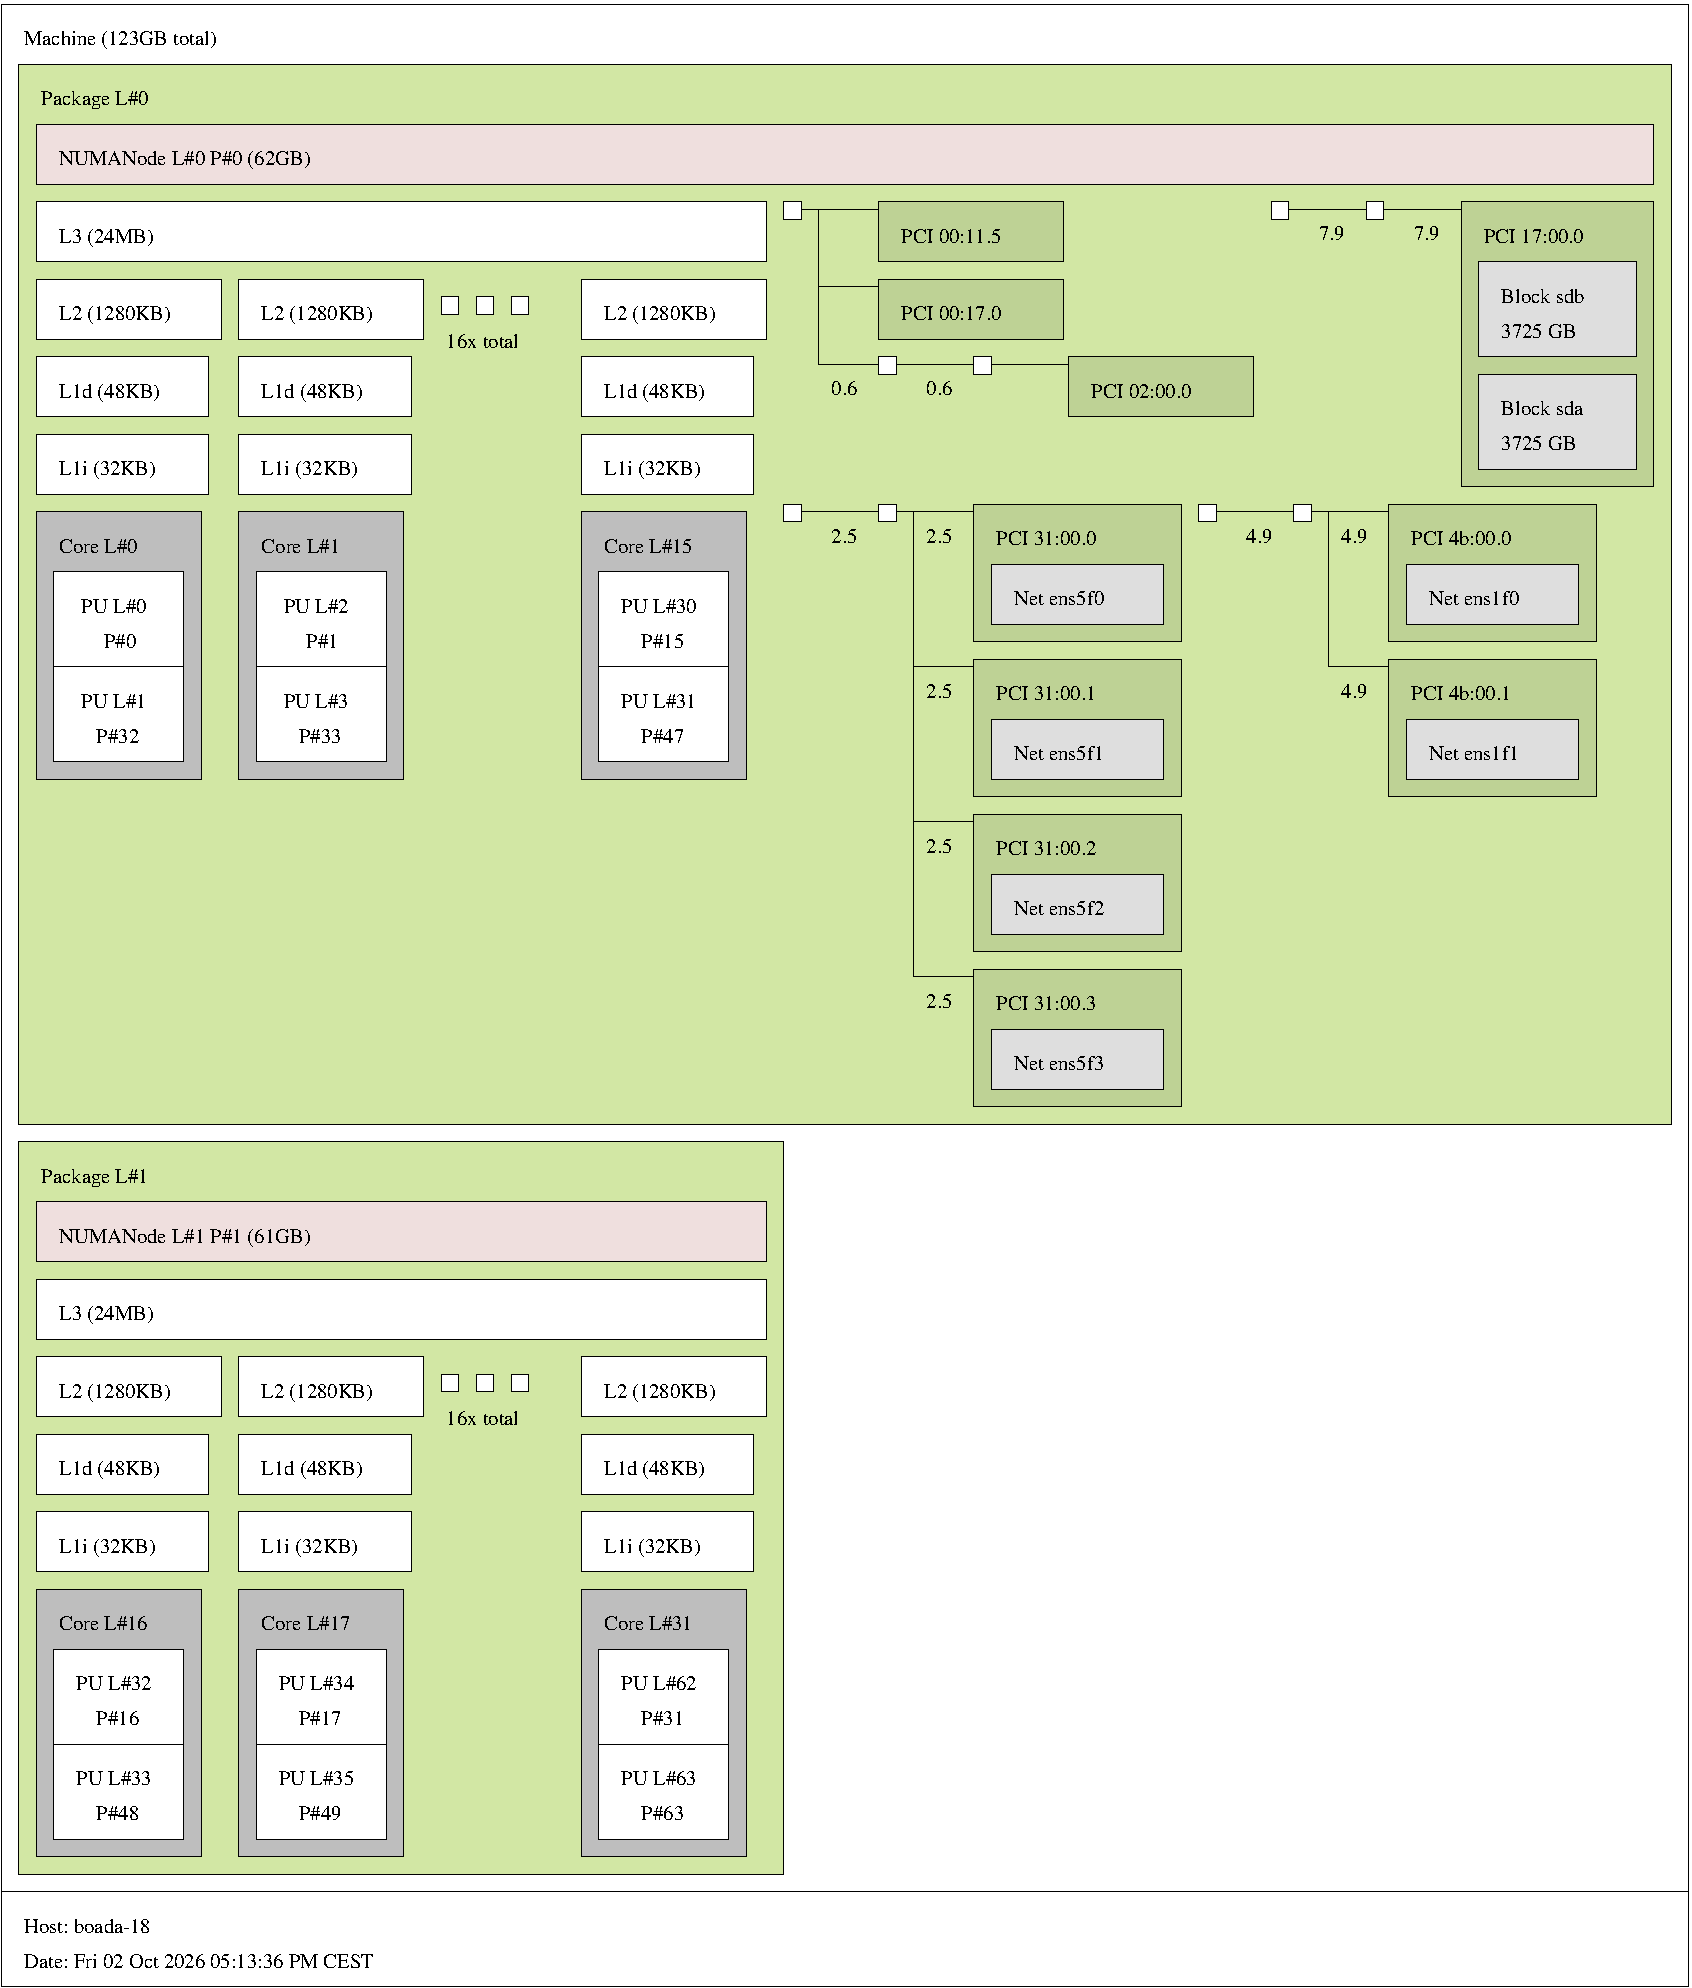
\includegraphics[width=\textwidth]{map-boada-18.pdf}
\caption{Topology diagram of boada-18 (\texttt{lstopo} output).}
\label{fig:topo}
\end{figure}


% ================================================================
\newpage
\section{Timing Sequential and Parallel Executions}
% ================================================================

% --------------------------------------------------
\subsection{OpenMP scaling (Question 3)}
% --------------------------------------------------

{\bfseries Strong scaling} keeps the problem size fixed ($10^9$ iterations) and increases the number of threads, so parallelism is used to reduce the execution time. The ideal speedup with $p$ threads is $p$. Figure~\ref{fig:omp-strong} shows that the time drops from $1.47$\,s with 1 thread to $0.047$\,s with 32 threads, a speedup of $30.99$ (efficiency $0.97$). The measured speedup tracks the ideal line almost perfectly up to 32 threads.

{\bfseries Weak scaling} grows the problem size proportionally with the number of threads ($10^8$ iterations per thread), so parallelism is used to solve a larger problem in the same time. The ideal is a constant execution time, i.e.\ an efficiency of 1. Figure~\ref{fig:omp-weak} shows the efficiency stays between $0.99$ and $1.00$ for all thread counts from 1 to 32.

The scalability is excellent in both scenarios because the iterations are independent, the only shared result is the reduction of \texttt{sum}, and the cyclic distribution gives every thread the same amount of work. The computation runs in registers, so there is no memory traffic or synchronization to limit it. The overhead of OpenMP itself is negligible: with 1 thread \texttt{pi\_omp} takes $1.4721$\,s against $1.4704$\,s for \texttt{pi\_seq} (speedup $0.999$).

{\bfseries Beyond 32 threads} (Figure~\ref{fig:omp-strong64}): boada-18 has 32 physical cores, so threads 33--64 run on the second hardware thread of a core that is already busy. With 33 threads the time jumps from $0.0476$\,s to $0.0906$\,s and the speedup falls from $30.8$ to $16.2$. Every thread receives the same amount of work, but the two threads sharing a core each run at about half speed, and the parallel region ends only when the slowest thread finishes. As more threads are added, each thread's share of work shrinks, so the time decreases again, but with 64 threads (two per core) it is $0.0483$\,s, no better than the $0.0476$\,s obtained with 32 threads.

The reason Hyper-Threading gives no gain is that \texttt{pi\_omp} is a \textbf{CPU-bound} application, not a memory-bound one. Hyper-Threading helps when a thread leaves the core idle while waiting for memory; here one thread already keeps the core's floating-point units busy, so a second thread on the same core only competes for the same resources.

\newpage
\begin{figure}[H]
\centering
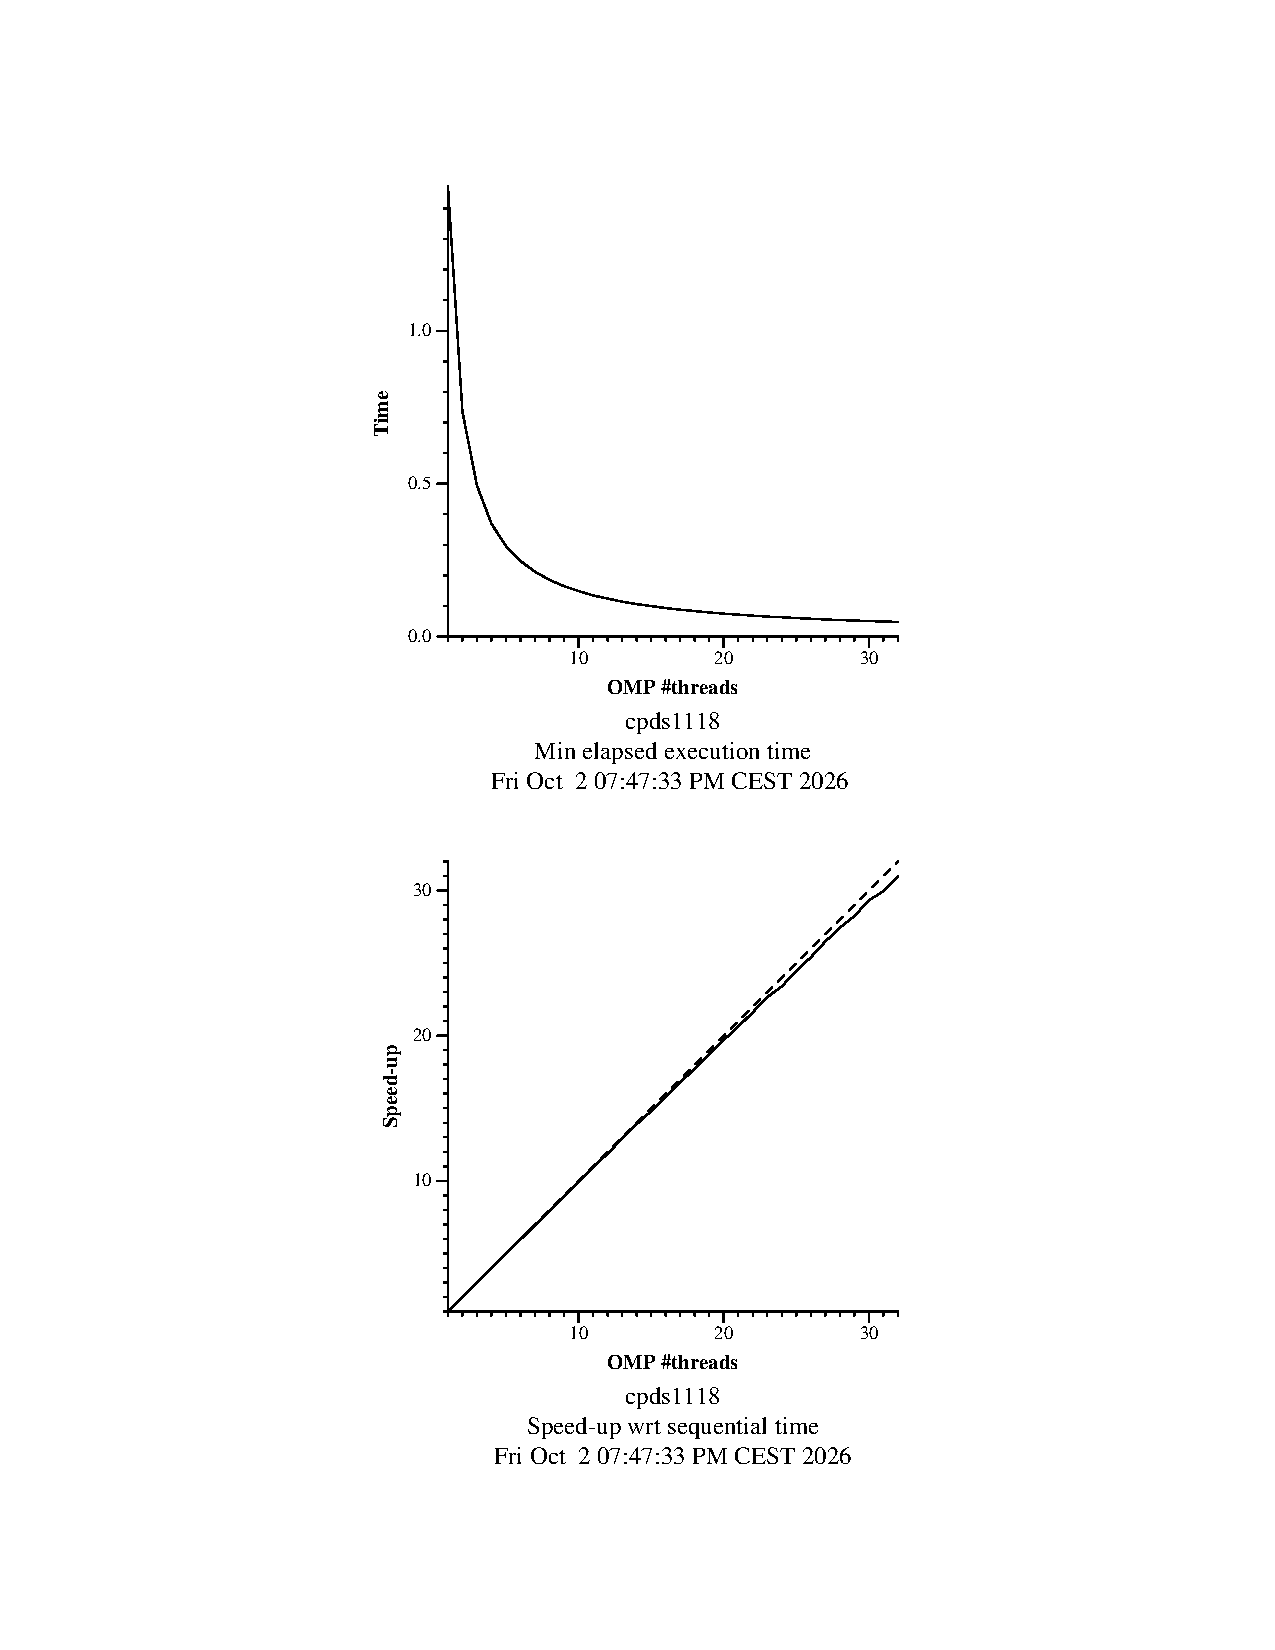
\includegraphics[width=0.75\textwidth]{pi_omp-1000000000-1-32-3-strong-boada-18.pdf}
\caption{OpenMP strong scaling: execution time and speed-up (1--32 threads, $10^9$ iterations).}
\label{fig:omp-strong}
\end{figure}

\begin{figure}[H]
\centering
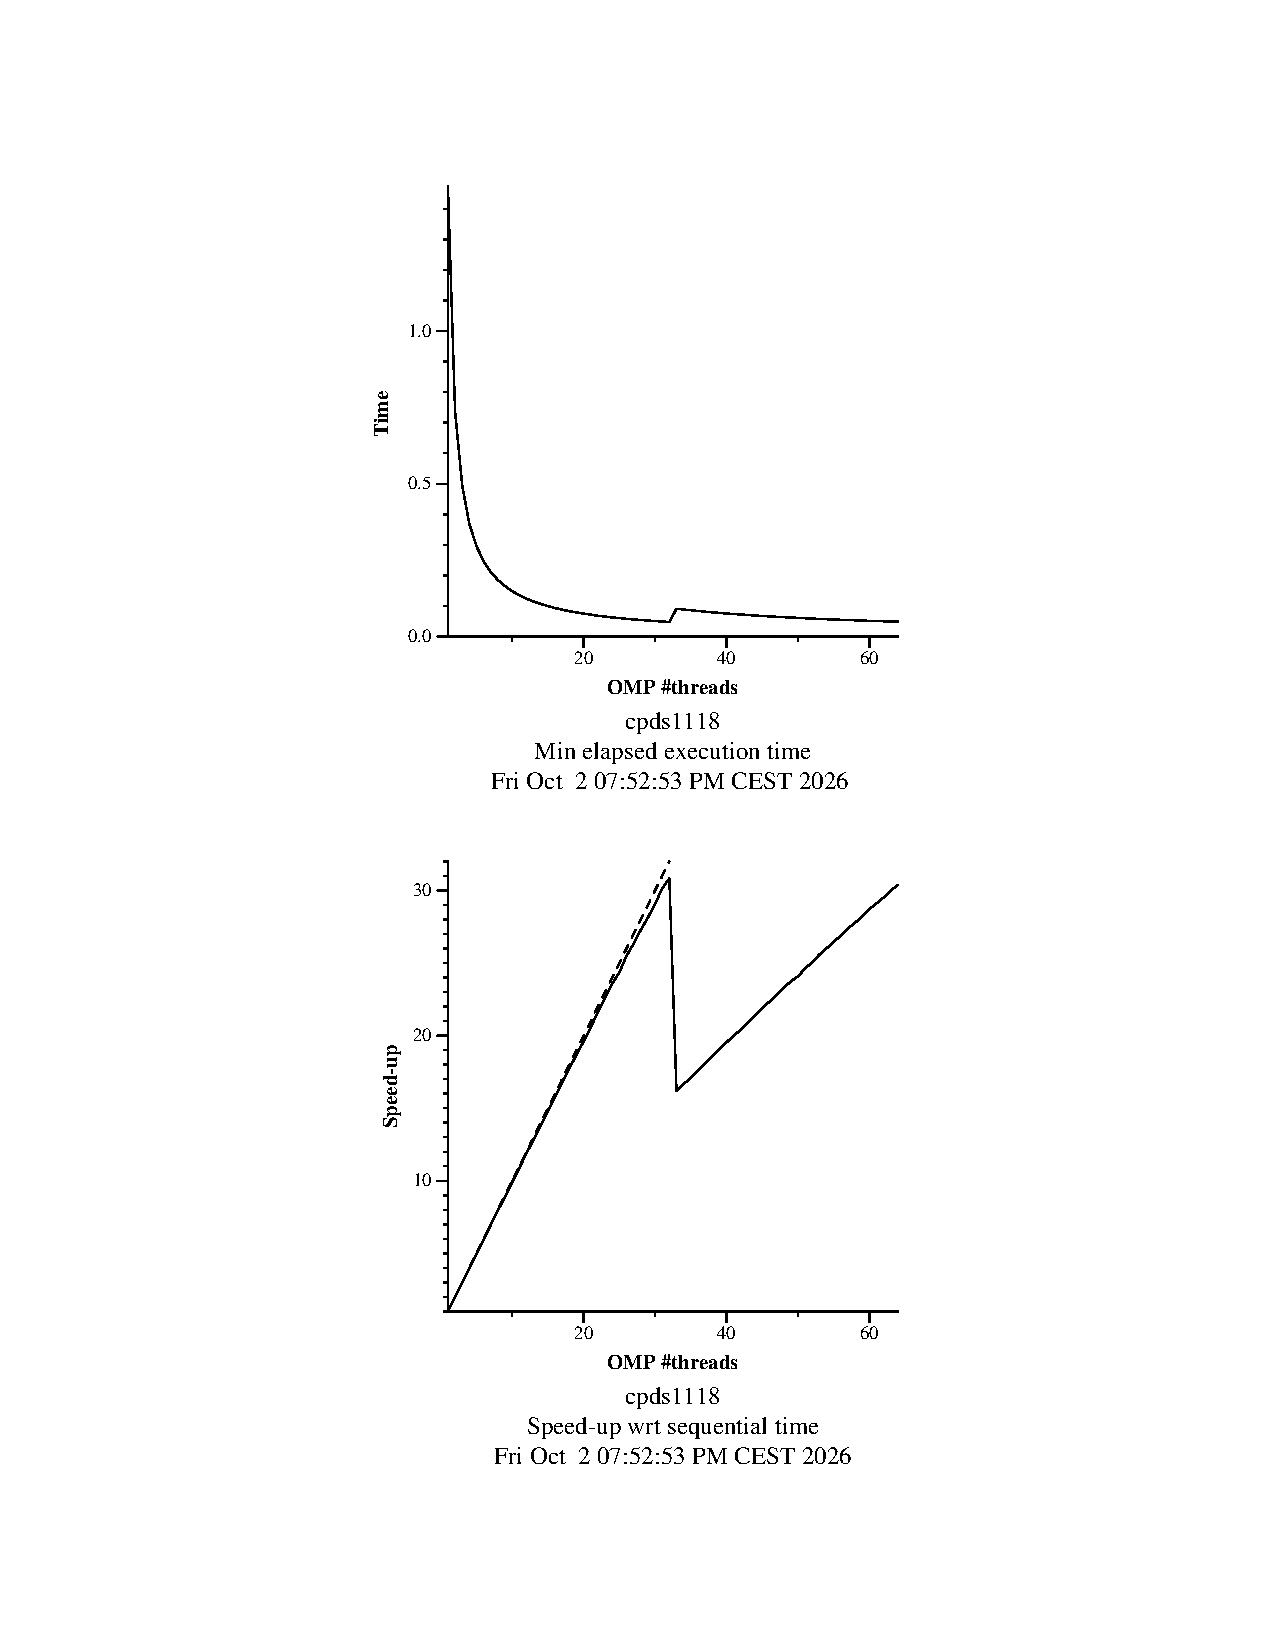
\includegraphics[width=0.75\textwidth]{pi_omp-1000000000-1-64-3-strong-boada-18.pdf}
\caption{OpenMP strong scaling: execution time and speed-up (1--64 threads, $10^9$ iterations).}
\label{fig:omp-strong64}
\end{figure}

\begin{figure}[H]
\centering
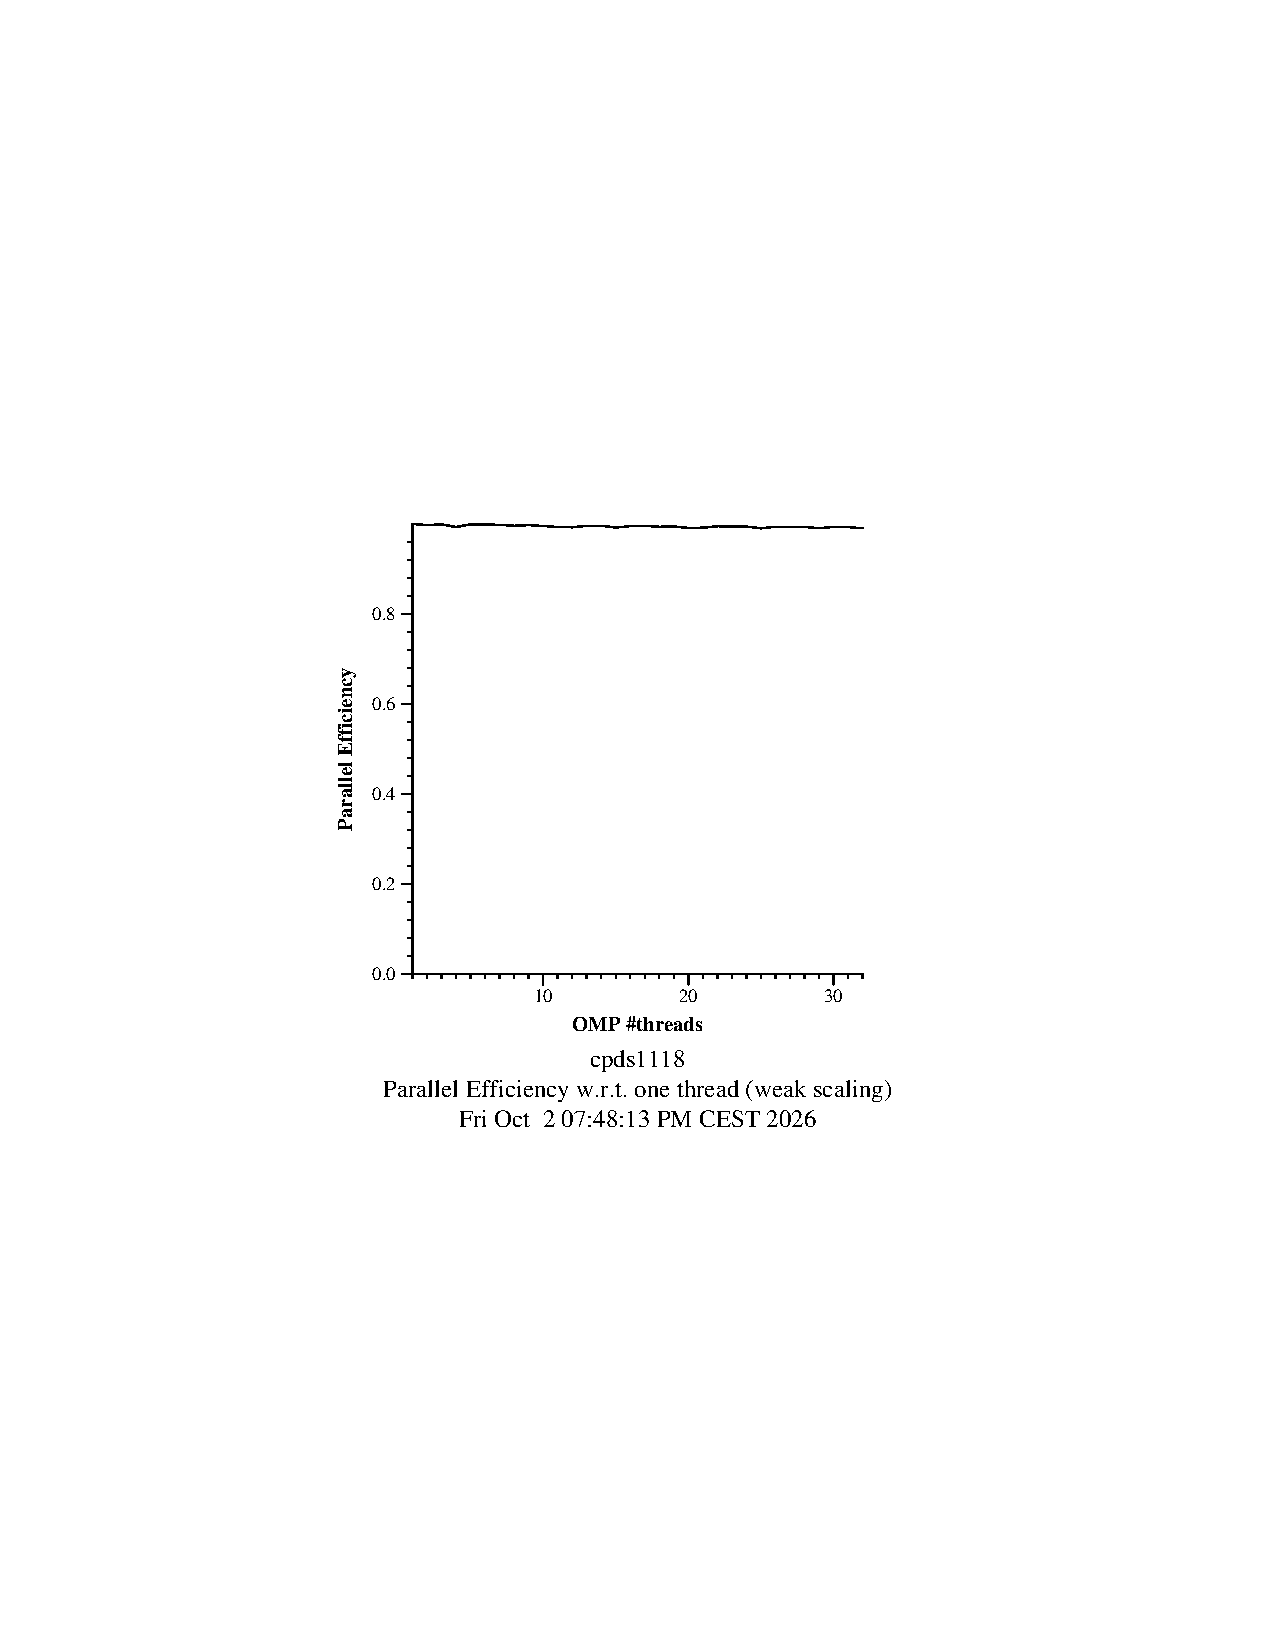
\includegraphics[width=0.75\textwidth]{pi_omp-100000000-1-32-3-weak-boada-18.pdf}
\caption{OpenMP weak scaling: parallel efficiency ($10^8$ iterations per thread).}
\label{fig:omp-weak}
\end{figure}


% --------------------------------------------------
\newpage
\subsection{MPI and hybrid scaling (Question 4)}
% --------------------------------------------------

\subsubsection{MPI strong scaling (1--32 processes)}

Figure~\ref{fig:mpi-strong} shows the execution time and speedup of the Monte Carlo code with 1 to 32 MPI processes. The execution scales well up to 16 processes and less well from 16 to 32.

With 1 process the speedup is $0.937$: the MPI program takes $11.79$\,s against $11.05$\,s for \texttt{pi\_seq}, a $6.7\%$ overhead. For OpenMP, the single-thread overhead was only $0.1\%$ (speedup $0.999$). MPI therefore introduces considerably more overhead than OpenMP, because it has to start processes and set up the communication layer, while OpenMP only creates threads inside one process.

Up to 16 processes the scaling is almost linear: 16 processes take $0.752$\,s, a speedup of $14.69$ over \texttt{pi\_seq} and an efficiency of $0.98$ relative to the 1-process MPI run. After that the curve bends. The time barely changes from 16 to 18 processes ($0.752$, $0.741$, $0.758$\,s), and from 16 to 32 processes it improves only by a factor of $1.73$ instead of 2. With 32 processes the time is $0.435$\,s, a speedup of $25.40$ and an efficiency of $0.79$.

This is explained by the allocation in \texttt{submit-strong-mpi.sh}: \texttt{--ntasks=1 --cpus-per-task=32} reserves 32 logical CPUs, which with 2 threads per core are 16 physical cores. Up to 16 processes each gets its own core. From the 17th process on, processes share cores through Hyper-Threading. At 17 and 18 processes only one or two cores are shared, and their processes become the slowest and set the total time. From 19 to 32 processes the sharing spreads over more cores and the time decreases again, but two processes on one core do not run as fast as two processes on two cores. Communication is not the bottleneck: the program performs only one \texttt{MPI\_Reduce} of a single value at the end.

\newpage

\begin{figure}[H]
\centering
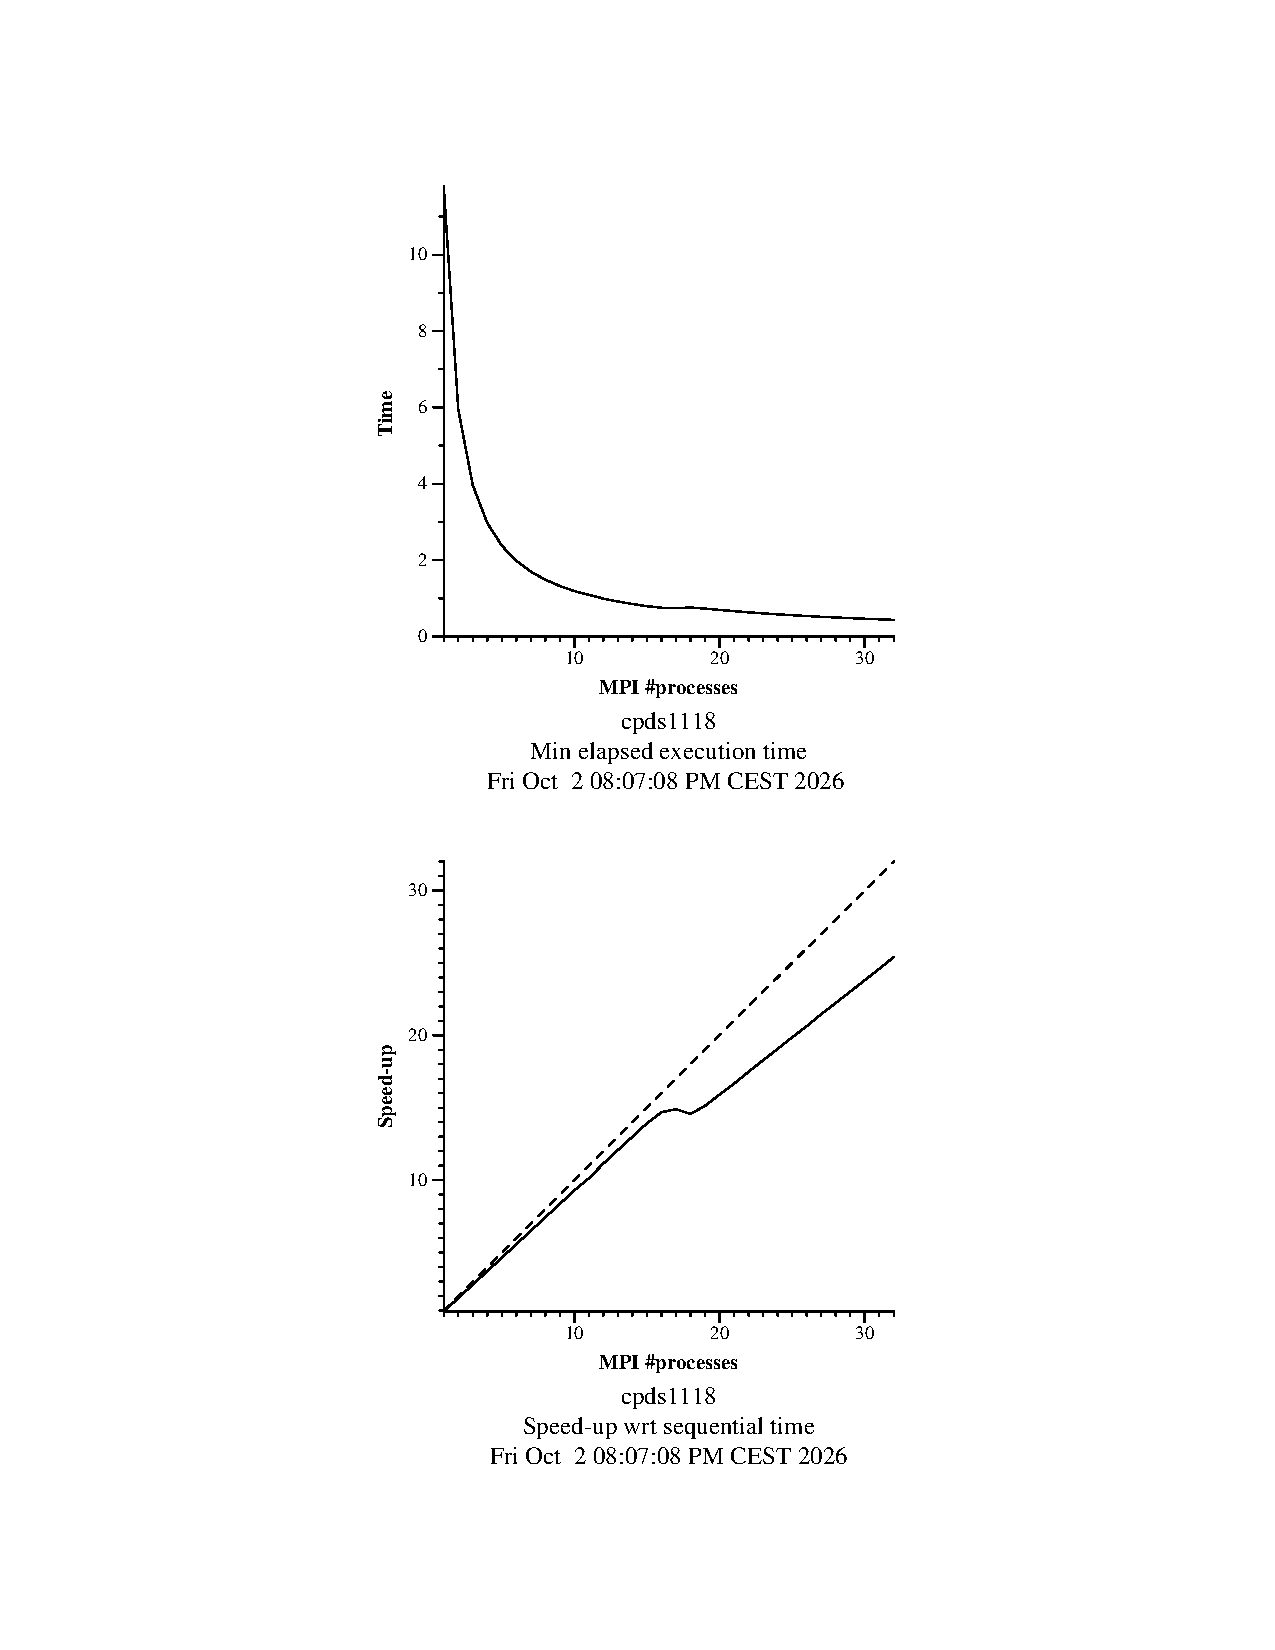
\includegraphics[width=0.75\textwidth]{pi_mpi_collectives-1073741824-1-32-3-strong-mpi-boada-18.pdf}
\caption{MPI strong scaling: execution time and speed-up (1--32 processes, $2^{30}$ iterations).}
\label{fig:mpi-strong}
\end{figure}


\newpage
\subsubsection{Hybrid MPI + OpenMP (2 processes, varying threads)}

Table~\ref{tab:hybrid} shows the elapsed time of \texttt{pi\_mpi\_omp} with 2 MPI processes and 1 to 32 OpenMP threads per process. The default run uses two nodes (one process on boada-18 and one on boada-19). The single-node run was made with \texttt{\#SBATCH --nodes=1}, and both processes ran on boada-18.

\begin{table}[H]
\centering
\begin{tabular}{rrr}
\toprule
\textbf{Total threads (2 MPI $\times$ threads)} & \textbf{Time, 2 nodes (s)} & \textbf{Time, 1 node (s)} \\
\midrule
 2 (2 $\times$  1) & 5.930 & 6.930 \\
 4 (2 $\times$  2) & 2.971 & 3.466 \\
 8 (2 $\times$  4) & 1.490 & 1.734 \\
16 (2 $\times$  8) & 0.751 & 0.867 \\
24 (2 $\times$ 12) & 0.497 & 0.578 \\
32 (2 $\times$ 16) & 0.373 & 0.434 \\
40 (2 $\times$ 20) & 0.299 & 0.348 \\
48 (2 $\times$ 24) & 0.249 & 0.292 \\
56 (2 $\times$ 28) & 0.213 & 0.249 \\
64 (2 $\times$ 32) & 0.187 & 0.219 \\
\bottomrule
\end{tabular}
\caption{Elapsed time for 2 MPI processes with varying OpenMP threads per process ($2^{30}$ iterations).}
\label{tab:hybrid}
\end{table}

\subsubsection{Summary of key execution times}

\begin{table}[H]
\centering
\begin{tabular}{lrrr}
\toprule
\textbf{Configuration} & \textbf{Time (s)} & \textbf{Speedup vs seq} & \textbf{Efficiency} \\
\midrule
Sequential (\texttt{pi\_seq})              & 11.05  & 1.00  & --- \\
32 MPI processes                           &  0.435 & 25.40 & 0.79 \\
2 MPI $\times$ 32 threads (2 nodes)        &  0.187 & 59.07 & 0.92 \\
2 MPI $\times$ 32 threads (1 node)         &  0.219 & 50.53 & 0.79 \\
\bottomrule
\end{tabular}
\caption{Comparison of key configurations ($2^{30}$ iterations). Efficiency is speedup divided by the number of processes $\times$ threads.}
\label{tab:summary}
\end{table}

\paragraph{32 MPI processes vs.\ 2 MPI $\times$ 16 threads.} With the same 32 workers, 32 MPI processes ($0.435$\,s) are slower than 2 processes with 16 threads each on two nodes ($0.373$\,s). The difference comes from the second node, not from MPI versus OpenMP: on a single node, 2 $\times$ 16 threads take $0.434$\,s, the same as 32 MPI processes. Spreading the work over two nodes gives every worker more hardware resources.

\paragraph{Speedup of 2 MPI $\times$ 32 threads.} On two nodes this configuration takes $0.187$\,s, a speedup of $11.05/0.187 = 59.07$ over the sequential Monte Carlo code (efficiency $0.92$ on 64 threads).

\paragraph{Comparison with OpenMP at 64 threads.} The result does not match Section~1.4.3. There, going from 32 to 64 OpenMP threads gave no improvement ($0.0476$\,s to $0.0483$\,s). Here, going from 2 $\times$ 16 to 2 $\times$ 32 threads halves the time, both on two nodes ($0.373$ to $0.187$\,s, $\times 2.00$) and on a single node ($0.434$ to $0.219$\,s, $\times 1.98$).

The single-node run proves that the improvement is not due to having more physical cores: on one node, 64 threads share 32 physical cores through Hyper-Threading, exactly as in the OpenMP 64-thread test, and the time still halves. The different behaviour comes from the code. \texttt{pi\_omp} keeps each core's floating-point units fully busy with one thread, so a second hardware thread has nothing to add. The Monte Carlo code is limited by latency instead: each call to \texttt{my\_rand} depends on the seed produced by the previous call, through a 64-bit multiplication and modulo. One thread spends most cycles waiting for the previous result, leaving the core's execution units idle, and the second hardware thread fills those idle cycles. Hyper-Threading therefore nearly doubles throughput for this code but not for \texttt{pi\_omp}.

Using one node instead of two makes every configuration about $17\%$ slower (ratio $1.16$--$1.17$ in all rows of Table~\ref{tab:hybrid}, including 2 $\times$ 1), so the 1-node 2 $\times$ 32 run takes $0.219$\,s instead of $0.187$\,s.

\end{document}
